\chapter{Adversarial Attacks: esperimenti}
\label{chap:4}

In questo capitolo si illustrano due applicazioni di grande successo per la classificazione di immagini mediche:
\begin{enumerate}
    \item classificazione delle malattie del torace attraverso radiografie (chest X-Ray) del torace.
    \item classificazione delle malattie dell'encefalo attraverso risonanze magnetiche cerebrali.
\end{enumerate}
Inoltre, si descrivono alcune impostazioni sperimentali generali rispetto ai dataset e alle architetture di rete presi in esame durante il lavoro di tesi. \\\\
Infine, si riportano i risultati degli esperimenti condotti sugli attacchi scelti. 
\newpage

\section{Datasets}

    \subsection{Chest X-Ray (Pneumonia) Dataset}
    
        \paragraph{Cos'è la polmonite?}
        La polmonite è una malattia infiammatoria che può colpire uno o entrambi i polmoni.
        
        \paragraph{Perché è importante?} 
        Secondo l'Organizzazione Mondiale della Sanità (OMS), la polmonite uccide circa 2 milioni di bambini sotto i 5 anni ogni anno ed è costantemente stimata come la principale causa di mortalità infantile \cite{rudan2008epidemiology}, uccidendo più bambini di HIV/AIDS, malaria e morbillo messi insieme \cite{adegbola2012childhood}.
        
        Gli agenti patogeni batterici e virali sono le due principali cause di polmonite ma richiedono forme di gestione molto diverse.
        La polmonite batterica richiede un ricovero urgente per un trattamento antibiotico immediato, mentre la polmonite virale viene trattata con cure di supporto.
        
        Pertanto, una diagnosi accurata e tempestiva è imperativa per facilitare i ricoveri rapidi per i bambini che hanno bisogno di un intervento urgente. 
        
        \paragraph{Informazioni sul dataset}
        Il dataset \cite{Chest_X_Ray_Dataset} contiene 5863 immagini di radiografie di toraci di bambini suddivise in \textbf{2 classi}:
            \begin{itemize}
                \item \textbf{Normal}
                \item \textbf{Pneumonia} (o \textit{Polmonite}): ogni infiammazione, acuta o cronica del parenchima polmonare, causata principalmente da agenti patogeni batterici o virali.
            \end{itemize}
        
        Ad ogni immagine del dataset è assosciata una sola classe.\\\\
        Di seguito alcuni esempi di immagini contenute nel dataset:
            \begin{figure}[!ht]
                \centering
                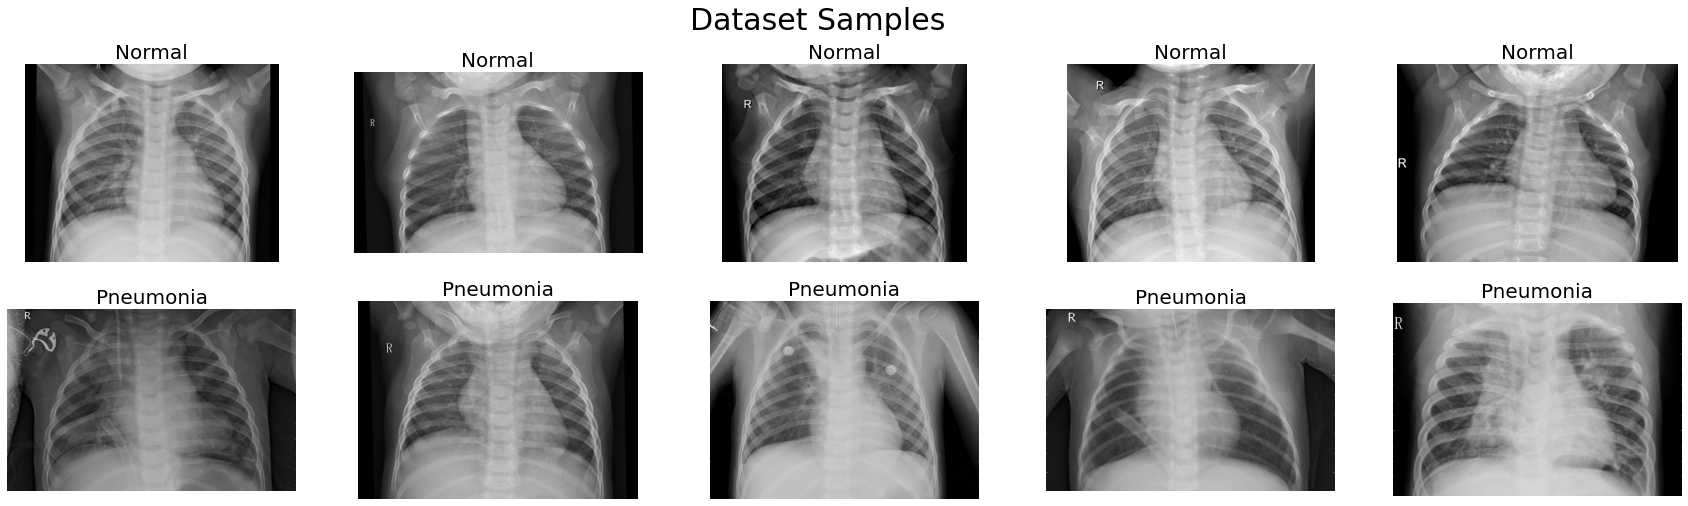
\includegraphics[width=\textwidth]{Images/Datasets/Pneumonia Dataset Samples.png}
                \caption{10 esempi di immagini presenti nel dataset \textit{Chest X-Ray}. I 5 esempi superiori aventi classe \textit{normal}, i 5 inferiori aventi classe \textit{pneumonia}.}
                \label{Pneumonia Samples}
            \end{figure}
    \newpage
    
    \subsection{Brain Tumor MRI Dataset}
    
        \paragraph{Cos'è un tumore cerebrale?}
        Un tumore al cervello è una massa di cellule, formatasi e cresciuta in modo del tutto anomalo all'interno dell'encefalo.
        
        I tumori al cervello, o tumori cerebrali, vengono classificati in base a più criteri, come la sede in cui comincia la crescita della massa tumorale e la velocità di diffusione (invasività) di quest'ultima.
        
        \paragraph{Perché è importante?}
        Il tumore al cervello è considerato una delle malattie più aggressive tra bambini e adulti. %\cite{Brain_Tumor_statistics}. 
        I tumori al cervello rappresentano l'85-90$\%$ di tutti i tumori primari del sistema nervoso centrale (SNC). Ogni anno, a circa 25.000 persone viene diagnosticato un tumore al cervello. Il tasso di sopravvivenza a 5 anni dalla diagnosi per le persone con un tumore al cervello o al SNC è di circa il 34$\%$ per gli uomini e il 36$\%$ per le donne.
        
        Trattamenti adeguati e ben pianificati, e una diagnosi accurata sono fondamentali per migliorare l'aspettativa di vita dei pazienti.
        
        La migliore tecnica per rilevare i tumori cerebrali è la risonanza magnetica (MRI). Un'enorme quantità di dati, sotto forma di immagini, viene generata attraverso le scansioni. Queste immagini vengono poi esaminate dai radiologi. Ma un esame manuale può essere soggetto ad errori a causa del livello di complessità dei tumori cerebrali e delle loro proprietà.
        
        L'applicazione di tecniche di classificazione automatizzata utilizzando l'apprendimento automatico (ML) e l'intelligenza artificiale (AI) ha dimostrato una maggiore accuratezza rispetto alla classificazione manuale.
        
        \paragraph{Informazioni sul dataset}
        Il dataset \cite{Brain_Tumor_MRI_Dataset} contiene 7022 immagini di risonanze magnetiche cerebrali umane suddivise in \textbf{4 classi}:
            \begin{itemize}
                \item \textbf{Glioma}: un tumore che si sviluppa a partire dalle cellule della glia (o cellule gliali) del sistema nervoso centrale
                \item \textbf{Meningioma}: un tumore cerebrale che origina dalle meningi, ovvero le membrane protettive che circondano e proteggono il cervello e il midollo spinale.
                \item \textbf{No tumor}
                \item \textbf{Pituitary}: un adenoma ipofisario, anche conosciuto come adenoma pituitario, è un tumore generalmente benigno che colpisce l’ipofisi, una ghiandola dalle dimensioni molto ridotte che si trova sotto l’ipotalamo
            \end{itemize}
        
        Ad ogni immagine del dataset è assosciata una sola classe.\\\\
        \newpage
        Di seguito alcuni esempi di immagini contenute nel dataset:
            \begin{figure}[!h]
                \centering
                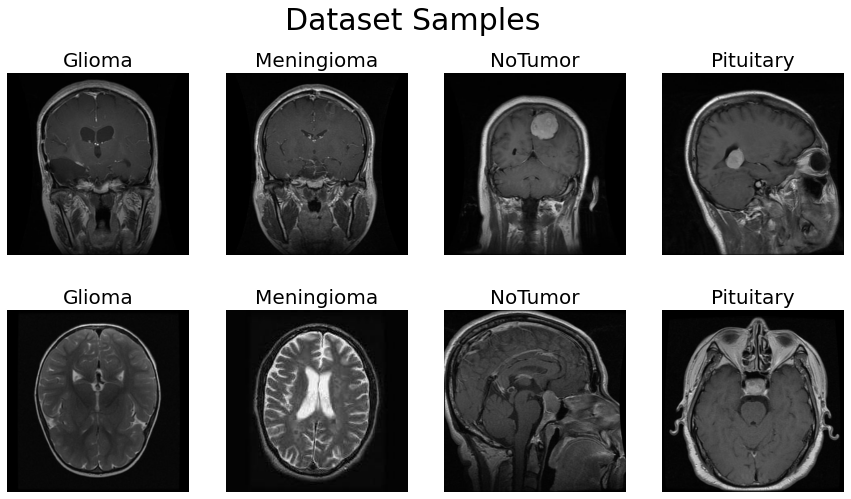
\includegraphics[width=\textwidth]{Images/Datasets/Brain Dataset Samples.png}
                \caption{8 esempi di immagini presenti nel dataset \textit{Brain Tumor MRI} con rispettive classi.}
                \label{Brain Samples}
            \end{figure}
        \newpage
        
    \subsection{Tecniche di Training}
            \paragraph{Hold-Out method}
            \label{Hold-Out method}
            Questo è il metodo utilizzato durante il lavoro di tesi.
            
            Il dataset viene diviso casualmente in 3 subdatasets seguendo le seguenti proporzioni:
                \begin{itemize}
                    \item Training dataset: $70\%$
                    \item Validation dataset: $20\%$
                    \item Testing dataset: $10\%$
                \end{itemize}
            
            \paragraph{Cross-validation method}
            
                \begin{itemize}
                    \item \textbf{k-fold method}: il dataset viene diviso casualmente in $k$ subdatasets di uguali dimensioni. Dei $k$ subdatasets solo uno viene scelto come Validation dataset, i restanti $k-$1 si concatenano per formare il Training dataset. Il processo viene ripetuto $k$ volte, con ciascuno dei $k$ subdatasets utilizzato solo una volta come Validation dataset.\\
                    Dopo aver calcolato i $k$ risultati finali si elabora la media per produrre una singola stima.\\
                    Comunemente si attribuisce $k=10$, ma in generale rimane un parametro non fissato. 
                        \begin{figure}[!h]
                            \centering
                            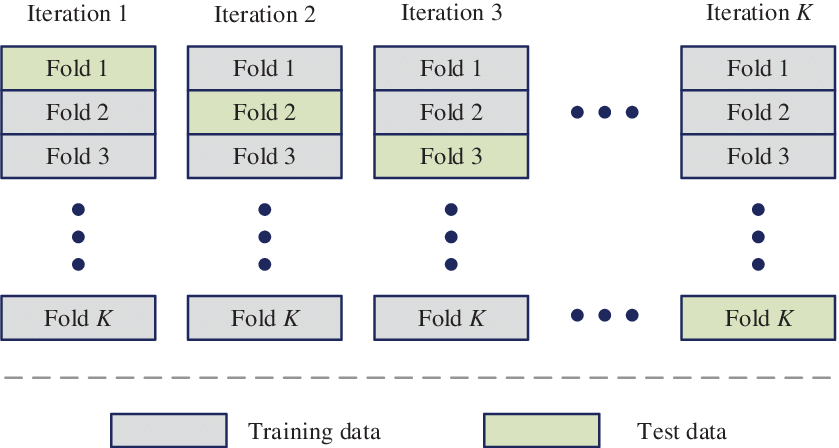
\includegraphics[width=0.7\textwidth]{Images/Datasets/K-fold-cross-validation-method.png}
                            \label{K-fold-cross-validation}
                            \caption{K-fold Cross-validation method}
                        \end{figure}
                    \item \textbf{n-fold method} (o \textbf{leave-one-out method}): Metodo simile al k-fold method.
                    Sia $n$ il numero di campioni all'interno del dataset, quest'ultimo viene diviso in $n$ subdatasets di dimensione 1, ognuno dei quali contiene uno e un solo campione del dataset.
                \end{itemize}
                
                Il vantaggio di questo metodo rispetto al \textit{Hold-Out method} è che tutti i campioni del dataset sono usati sia per il training che per la validation, e ogni campione è usato per la validation esattamente una volta. Per questo motivo il metodo aiuta a determinare una stima più accurata delle prestazioni di previsione del modello.
                Lo svantaggio è che il modello viene trainato $k$ volte e, in caso di datasets di dimensioni molto elevate, ciò può risultare estremamente costoso a livello computazionale.\\\\
            Durante il lavoro di tesi sono state provate entrambe le tecniche di training ma è stato scelto l'\textit{Hold-Out method} poiché, nonostante il \textit{k-fold cross-validation method} richieda un maggiore impiego di tempo e risorse a livello computazionale, non è stato in grado di ottenere un miglioramento significativo dei risultati.
                
\newpage        

\section{Modelli}

    \paragraph{Cos'è un modello pre-trainato e perché utilizzarlo}
    Un modello pre-trainato è un modello precedentemente trainato su un set di dati contenente \textit{weights} e \textit{biases} rappresentanti caratteristiche di quello specifico dataset. Se il dataset è abbastanza grande le caratteristiche apprese saranno molto probabilmente trasferibili su dataset differenti.
    
    L'utilizzo di un modello pre-trainato risulta vantaggioso perché permette di risparmiare tempo. Tempo e risorse di calcolo sono già state spese per permettere al modello di imparare caratteristiche fondamentali.\\
    
    Per il lavoro di tesi sono stati utilizzati 5 modelli CNN pre-trainati sul dataset ImageNet \cite{deng2009imagenet}, contenente più di 14 milioni di immagini divise in più di 20.000 classi:
        \begin{itemize}
            \item DenseNet121
            \item ResNet152 
            \item VGG19
            \item MobileNetV2
            \item InceptionV3
        \end{itemize}
    \newpage
    
    \subsection{DenseNet121}
    \label{DenseNet121}
    Una Dense Convolutional Network (DenseNet) %[bibl: https://arxiv.org/abs/1608.06993]
    \cite{huang2016densely}, collega ogni strato ad ogni altro strato in maniera feed forward. Mentre le reti convoluzionali tradizionali con L strati hanno L connessioni (una tra ogni strato e il suo successivo) una DenseNet ha L(L+1)/2 connessioni dirette. Per ogni strato, le feature-map di tutti gli strati precedenti sono usate come input, e le sue stesse feature-map sono usate come input in tutti gli strati successivi. 
    
    Le DenseNets hanno diversi vantaggi: alleviano il problema del vanishing-gradient, migliorano la propagazione delle features, incoraggiano il riutilizzo delle features e riducono sostanzialmente il numero di parametri.
        
        \paragraph{Architettura}
        Di seguito l'architettura del modello DenseNet121:
            \begin{table}[!h]
                \centering
                \begin{tabular}{|c|c|c|}
                    \hline 
                    \rule[-3mm]{0mm}{8mm}
                    \textbf{Layers} & \textbf{Output Size} & \textbf{DenseNet-121} \\
                    \hline \hline
                    \rule[-3mm]{0mm}{8mm}
                    Convolution & 112 $\times$ 112 & 7 $\times$ 7 conv, stride 2 \\
                    \hline 
                    \rule[-3mm]{0mm}{8mm}
                    Pooling & 56 $\times$ 56 & 3 $\times$ 3 max pool, stride 2\\
                    \hline 
                    \rule[-6mm]{0mm}{1.4cm}
                    Dense Block  (1) & 56 $\times$ 56 & $\begin{bmatrix} 1 \times 1  \hspace{.2cm} \text{conv}\\ 3 \times 3 \hspace{.2cm} \text{conv} \end{bmatrix} \times 6 $ \\
                    \hline
                    \rule[-3mm]{0mm}{8mm}
                    Transition Layer (1) & 56 $\times$ 56 & 1 $\times$ 1 conv \\
                    \cline{2-3}
                    \rule[-3mm]{0mm}{8mm}
                    & 28 $\times$ 28 & 2 $\times$ 2 avarage pool, stride 2\\
                    \hline 
                    \rule[-6mm]{0mm}{1.4cm}
                    Dense Block  (2) & 28 $\times$ 28 & $\begin{bmatrix} 1 \times 1  \hspace{.2cm} \text{conv}\\ 3 \times 3 \hspace{.2cm} \text{conv} \end{bmatrix} \times 12 $ \\
                    \hline
                    \rule[-3mm]{0mm}{8mm}
                    Transition Layer (2) & 28 $\times$ 28 & 1 $\times$ 1 conv \\
                    \cline{2-3}
                    \rule[-3mm]{0mm}{8mm}
                    & 14 $\times$ 14 & 2 $\times$ 2 avarage pool, stride 2\\
                    \hline 
                    \rule[-6mm]{0mm}{1.4cm}
                    Dense Block  (3) & 14 $\times$ 14 & $\begin{bmatrix} 1 \times 1  \hspace{.2cm} \text{conv}\\ 3 \times 3 \hspace{.2cm} \text{conv} \end{bmatrix} \times 24 $ \\
                    \hline
                    \rule[-3mm]{0mm}{8mm}
                    Transition Layer (3) & 14 $\times$ 14 & 1 $\times$ 1 conv \\
                    \cline{2-3}
                    \rule[-3mm]{0mm}{8mm}
                    & 7 $\times$ 7 & 2 $\times$ 2 avarage pool, stride 2\\
                    \hline 
                    \rule[-6mm]{0mm}{1.4cm}
                    Dense Block  (4) & 7 $\times$ 7 & $\begin{bmatrix} 1 \times 1  \hspace{.2cm} \text{conv}\\ 3 \times 3 \hspace{.2cm} \text{conv} \end{bmatrix} \times 16 $ \\
                    \hline
                    \rule[-3mm]{0mm}{8mm}
                    Classification Layer & 1 $\times$ 1 & 7 $\times$ 7 global avarage pool \\
                    \cline{2-3}
                    \rule[-3mm]{0mm}{8mm}
                    &  & 1000D fully-connected, softmax\\
                    \hline
                \end{tabular}
                \label{DenseNet121 Architecture}
            \end{table}
        
        \newpage
        
        \paragraph{Training and Validation Phase} 
        Di seguito sono riportati i grafici, prodotti durante il lavoro di tesi, raffiguranti le performance del modello, ovvero i valori dell'\textbf{accuracy} e della \textbf{loss} in funzione delle epoche, sia per la fase di \textit{Training} che di \textit{Validation}:
            \begin{figure}[!h]
                \centering
                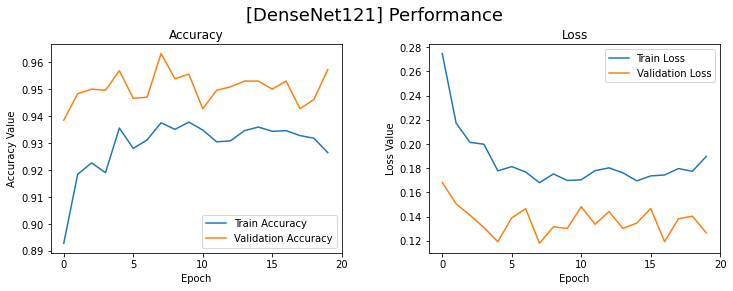
\includegraphics [width=\textwidth]{Images/Modelli/DenseNet121/DenseNet121 Pneumonia Performance.png}
                \caption{Performance durante le fasi di \textit{Training} e \textit{Validation} del modello \textit{DenseNet121} sui Training e Validation datasets di \textit{Chest X-Ray}}
                \label{DenseNet121 Pneumonia Performance}
            \end{figure}
            
            \begin{figure}[!h]
                \centering
                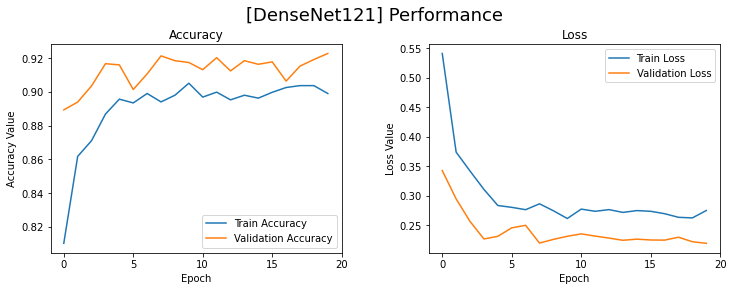
\includegraphics [width=\textwidth]{Images/Modelli/DenseNet121/DenseNet121 Brain Performance.png}
                \caption{Performance durante le fasi di \textit{Training} e \textit{Validation} del modello \textit{DenseNet121} sui Training e Validation datasets di \textit{Brain Tumor MRI}}
                \label{DenseNet121 Brain Performance}
            \end{figure}
        
        \newpage
        
        \paragraph{Testing Phase}
        Di seguito si riportano le Confusion Matrices e alcuni esempi di predizioni rispetto alle classi reali delle immagini, prodotti durante il lavoro di tesi:
            \begin{figure}[!h]
                \centering
                \subfloat[][Confusion Matrix del modello \textit{DenseNet121} sul Testing dataset di \textit{Chest X-Ray}] {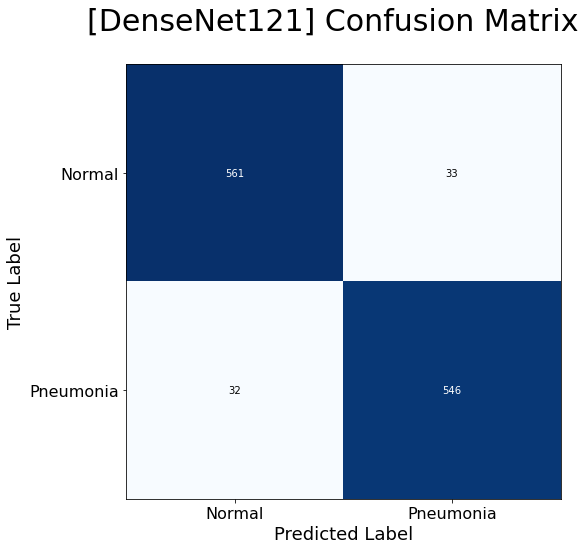
\includegraphics[width=.35\textwidth]{Images/Modelli/DenseNet121/DenseNet121 Pneumonia Confusion Matrix.png}} 
                \quad
                \subfloat[][Confusion Matrix del modello \textit{DenseNet121} sul Testing dataset di \textit{Brain Tumor MRI}] {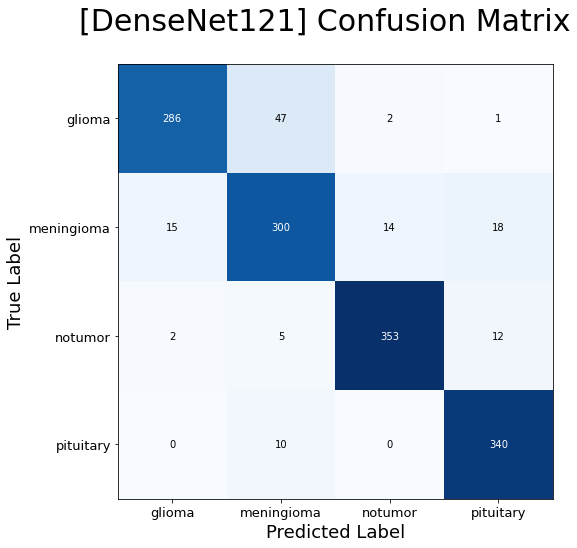
\includegraphics[width=.35\textwidth]{Images/Modelli/DenseNet121/DenseNet121 Brain Confusion Matrix.png}}
                \quad
                \subfloat[][10 esempi con rispettive classi reali e predizioni del modello \textit{DenseNet121} su immagini pulite del Testing dataset di \textit{Chest X-Ray}] {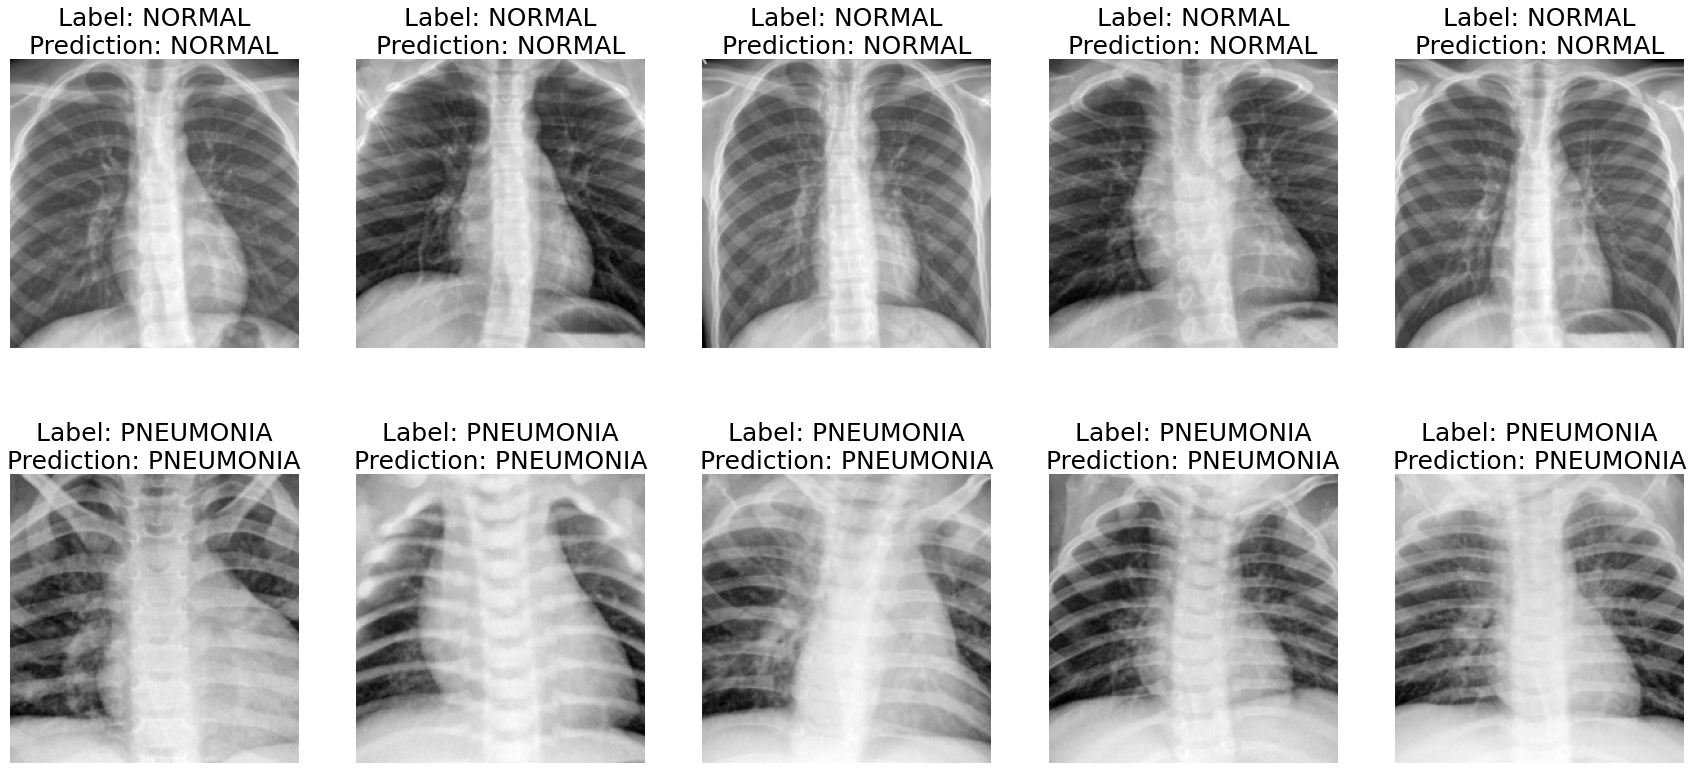
\includegraphics[width=.75\textwidth]{Images/Modelli/DenseNet121/DenseNet121 Pneumonia 10 True&Predictions.png}} \quad
                \subfloat[][8 esempi con rispettive classi reali e predizioni del modello\\ \textit{DenseNet121} su immagini pulite del Testing dataset di \textit{Brain Tumor MRI}] {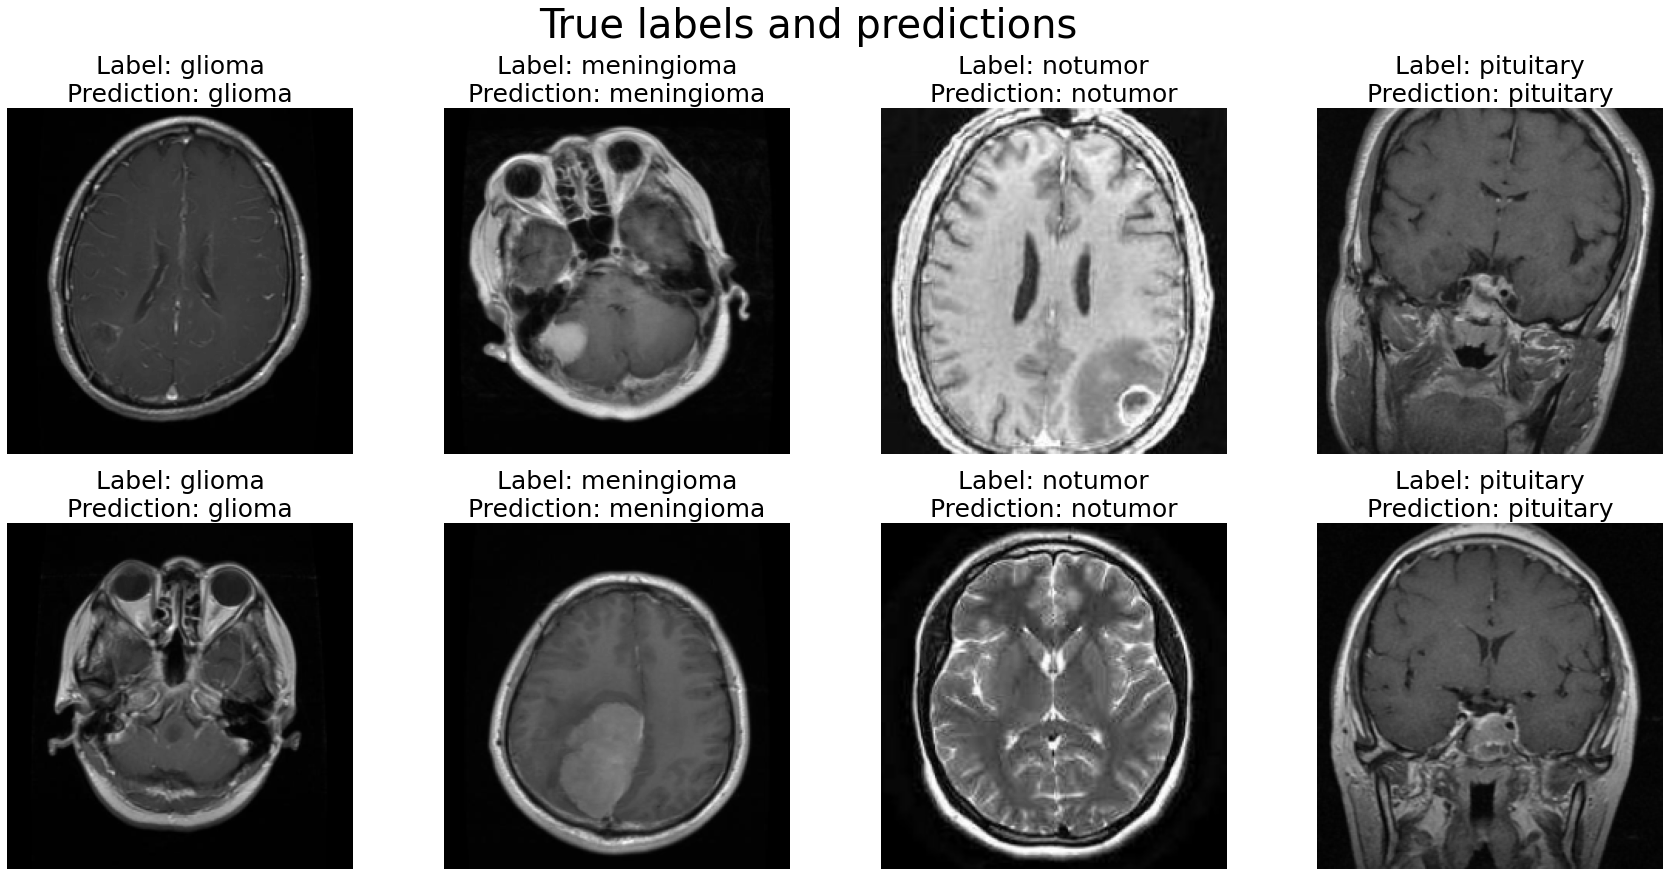
\includegraphics[width=.75\textwidth]{Images/Modelli/DenseNet121/DenseNet121 Brain 8 True&Predictions.png}}
                \caption{}
                \label{DenseNet121 Confusion Matrix and Predictions}
            \end{figure}
        \newpage
   
    \subsection{ResNet152}
    \label{ResNet152} 
    Una Residual Network (ResNet) \cite{he2015deep} limita la perdita di gradiente negli strati più profondi aggiungendo una connessione residua tra ogni strato di convoluzione.
        \begin{figure}[!h]
            \centering
            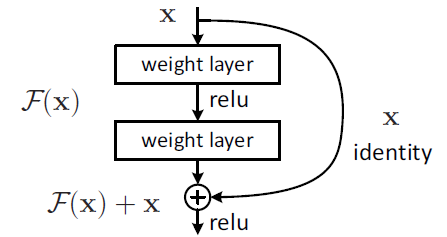
\includegraphics[width=0.5\textwidth]{Images/Modelli/ResNet152/Residual Connection.png}
            \caption{Residual Connection}
            \label{Residual Connection}
        \end{figure}
    
        \paragraph{Architettura}
        Di seguito l'architettura del modello ResNet152:
            \begin{table}[!h]
                \centering
                \begin{tabular}{|c|c|c|}
                \hline
                \rule[-3mm]{0mm}{8mm}
                \textbf{Layers}  & \textbf{Output Size} & \textbf{ResNet152} \\
                \hline \hline
                \rule[-3mm]{0mm}{8mm}
                conv 1 & 112 $\times$ 112 & 7 $\times$ 7, 64, stride 2 \\
                \hline
                \rule[-3mm]{0mm}{8mm}
                & & 3 $\times$ 3 max pool, stride 2\\
                \cline{3-3}
                \rule[-8mm]{0mm}{1.8cm}
                conv 2\textunderscore x & 56 $\times$ 56 &  $\begin{bmatrix} 1 \times 1, 64 \\  3 \times 3,  64 \\ 1 \times 1,  256 \end{bmatrix} \times 3 $ \\
                \hline
                \rule[-8mm]{0mm}{1.8cm}
                conv 3\textunderscore x & 28 $\times$ 28 &  $\begin{bmatrix} 1 \times 1, 128 \\  3 \times 3,  128 \\ 1 \times 1,  512 \end{bmatrix} \times 8 $ \\
                \hline
                \rule[-8mm]{0mm}{1.8cm}
                conv 4\textunderscore x & 14 $\times$ 14 &  $\begin{bmatrix} 1 \times 1, 256 \\  3 \times 3,  256 \\ 1 \times 1,  1024 \end{bmatrix} \times 36 $ \\
                \hline
                \rule[-8mm]{0mm}{1.8cm}
                conv 5\textunderscore x & 7 $\times$ 7  &  $\begin{bmatrix} 1 \times 1, 512 \\  3 \times 3,  512 \\ 1 \times 1,  2048 \end{bmatrix} \times 3 $ \\
                \hline
                \rule[-3mm]{0mm}{8mm}
                & 1 $\times$ 1 & average pool, 1000-d fc, softmax\\
                \hline
                \multicolumn{2}{|c|}{FLOPs} & \rule[-3mm]{0mm}{8mm}$11.3 \times 10^9$\\
                \hline
                \end{tabular}
               \label{ResNet152 Architecture}
            \end{table}
        \newpage
        
        \paragraph{Training and Validation Phase} 
        Di seguito sono riportati i grafici, prodotti durante il lavoro di tesi, raffiguranti le performance del modello, ovvero i valori dell'\textbf{accuracy} e della \textbf{loss} in funzione delle epoche, sia per la fase di \textit{Training} che di \textit{Validation}:
            \begin{figure}[!h]
                \centering
                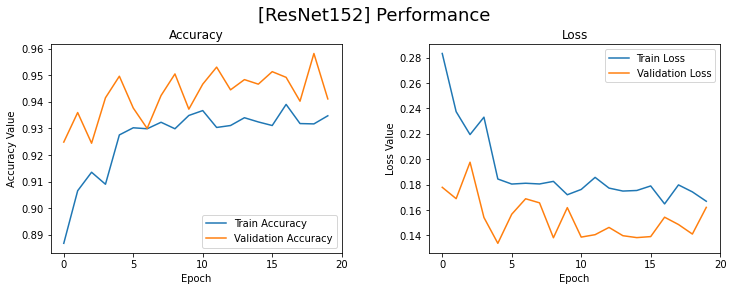
\includegraphics[width=0.7\textwidth]{Images/Modelli/ResNet152/ResNet152 Pneumonia Performance.png}
                \caption{Performance durante le fasi di \textit{Training} e \textit{Validation} del modello \textit{ResNet152} sui Training e Validation datasets di \textit{Chest X-Ray}}
                \label{ResNet152 Pneumonia Performance}
            \end{figure}
            
            \begin{figure}[!h]
                \centering
                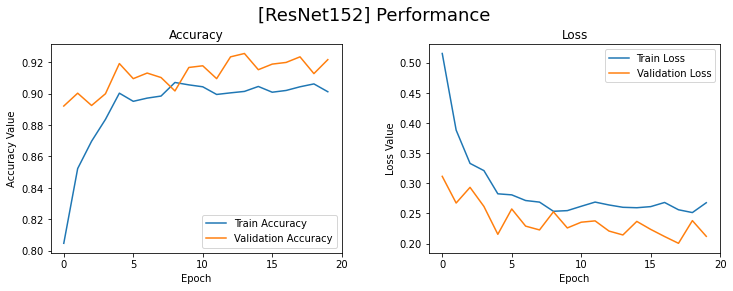
\includegraphics [width=0.7\textwidth]{Images/Modelli/ResNet152/ResNet152 Brain Performance.png}
                \caption{Performance durante le fasi di \textit{Training} e \textit{Validation} del modello \textit{ResNet152} sui Training e Validation datasets di \textit{Brain Tumor MRI}}
                \label{ResNet152 Brain Performance}
            \end{figure}
        
        \paragraph{Testing Phase}
        Di seguito si riportano le Confusion Matrices prodotte durante il lavoro di tesi:
            \begin{figure}[!h]
                \centering
                \subfloat[][Confusion Matrix del modello \textit{ResNet152} sul Testing dataset di \textit{Chest X-Ray}] {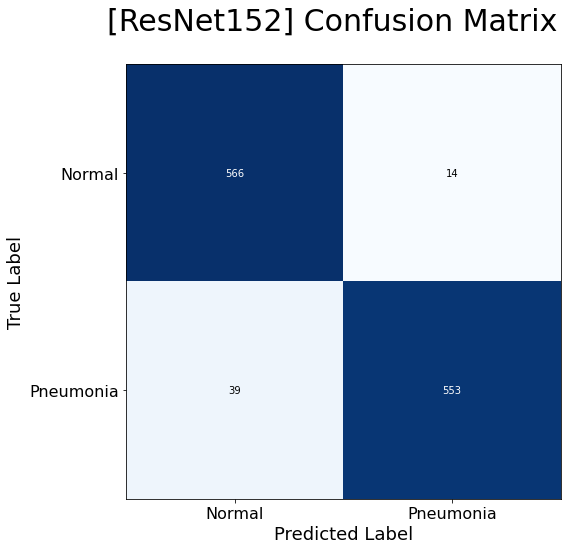
\includegraphics[width=.3\textwidth]{Images/Modelli/ResNet152/ResNet152 Pneumonia Confusion Matrix.png}} 
                \quad
                \subfloat[][Confusion Matrix del modello \textit{ResNet152} sul Testing dataset di \textit{Brain Tumor MRI}] {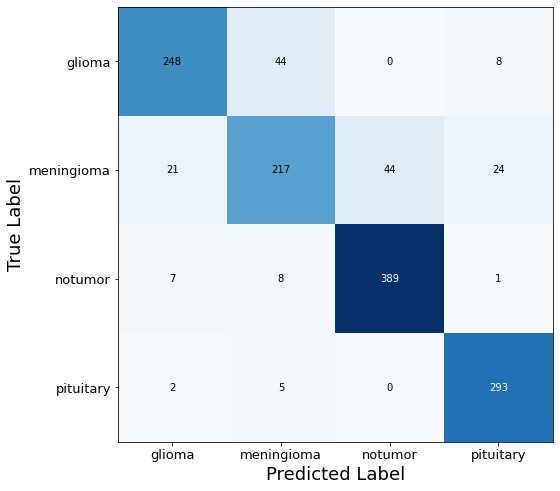
\includegraphics[width=.3\textwidth]{Images/Modelli/ResNet152/ResNet152 Brain Confusion Matrix.png}}
                \caption{}
                \label{ResNet152 Confusion Matrix}
            \end{figure}
        \newpage 
    
    \subsection{VGG19}
    \label{VGG19}
    
    %[bibl: arXiv:1409.1556]
    
        \paragraph{Architettura}
        Di seguito l'architettura del modello VGG19 \cite{simonyan2014very}:\\
            \begin{table} [!h]
                \centering
                \begin{tabular}{|c|}
                    \hline 
                    ConvNet Configuration\\
                    \hline \hline
                    \rule[-3mm]{0mm}{8mm}
                    \textbf{19 weight layers}\\
                    \hline
                    \hline
                    \rule[-3mm]{0mm}{8mm}
                    input ($224\times224$ RGB image)\\
                    \hline
                    conv3-64\\
                    conv3-64\\
                    \hline 
                    \rule[-3mm]{0mm}{8mm}
                    maxpool (1)\\
                    \hline 
                    conv3-128\\
                    conv3-128\\
                    \hline  
                    \rule[-3mm]{0mm}{8mm}
                    maxpool (2)\\
                    \hline 
                    conv3-256\\
                    conv3-256\\
                    conv3-256\\
                    conv3-256\\
                    \hline 
                    \rule[-3mm]{0mm}{8mm}
                    maxpool (3)\\
                    \hline 
                    conv3-512\\
                    conv3-512\\
                    conv3-512\\
                    conv3-512\\
                    \hline 
                    \rule[-3mm]{0mm}{8mm}
                    maxpool (4)\\
                    \hline 
                    conv3-512\\
                    conv3-512\\
                    conv3-512\\
                    conv3-512\\
                    \hline 
                    \rule[-3mm]{0mm}{8mm}
                    maxpool (5)\\
                    \hline 
                    \rule[-3mm]{0mm}{8mm}
                    FC-4096\\
                    \hline 
                    \rule[-3mm]{0mm}{8mm}
                    FC-4096\\
                    \hline 
                    \rule[-3mm]{0mm}{8mm}
                    FC-1000\\
                    \hline 
                    \rule[-3mm]{0mm}{8mm}
                    soft-max\\
                    \hline 
                \end{tabular}
            \end{table}
        \newpage
        
        \paragraph{Training and Validation Phase} 
        Di seguito sono riportati i grafici, prodotti durante il lavoro di tesi, raffiguranti le performance del modello, ovvero i valori dell'\textbf{accuracy} e della \textbf{loss} in funzione delle epoche, sia per la fase di \textit{Training} che di \textit{Validation}:
            \begin{figure}[!h]
                \centering
                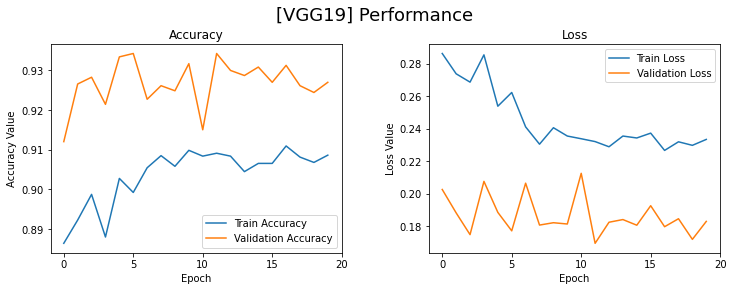
\includegraphics[width=0.7\textwidth]{Images/Modelli/VGG19/VGG19 Pneumonia Performance.png}
                \caption{Performance durante le fasi di \textit{Training} e \textit{Validation} del modello \textit{VGG19} sui Training e Validation datasets di \textit{Chest X-Ray}}
                \label{VGG19 Pneumonia Performance}
            \end{figure}
            
            \begin{figure}[!h]
                \centering
                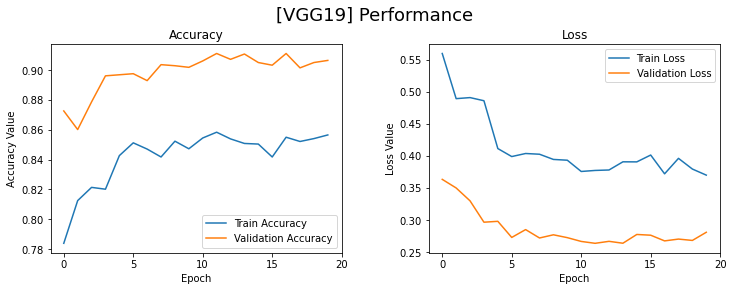
\includegraphics [width=0.7\textwidth]{Images/Modelli/VGG19/VGG19 Brain Performance.png}
                \caption{Performance durante le fasi di \textit{Training} e \textit{Validation} del modello \textit{VGG19} sui Training e Validation datasets di \textit{Brain Tumor MRI}}
                \label{VGG19 Brain Performance}
            \end{figure}
        
        \paragraph{Testing Phase}
        Di seguito si riportano le Confusion Matrices prodotte durante il lavoro di tesi:
            \begin{figure}[!h]
                \centering
                \subfloat[][Confusion Matrix del modello \textit{VGG19} sul Testing dataset di \textit{Chest X-Ray}] {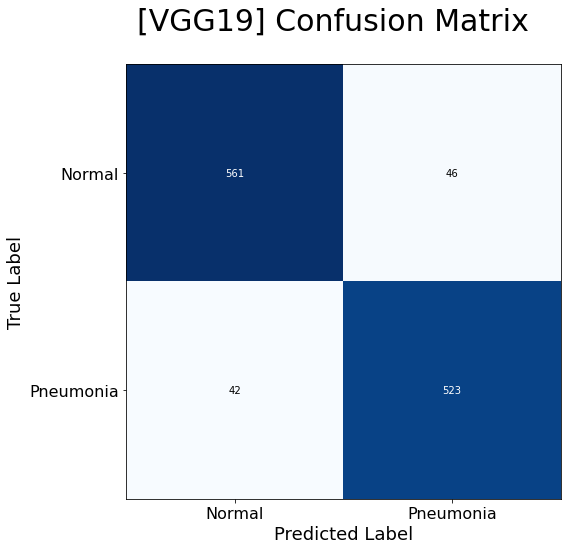
\includegraphics[width=.3\textwidth]{Images/Modelli/VGG19/VGG19 Pneumonia Confusion Matrix.png}} 
                \quad
                \subfloat[][Confusion Matrix del modello \textit{VGG19} sul Testing dataset di \textit{Brain Tumor MRI}] {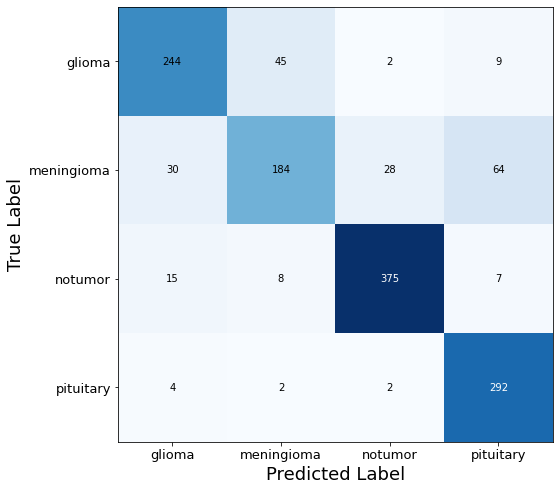
\includegraphics[width=.3\textwidth]{Images/Modelli/VGG19/VGG19 Brain Confusion Matrix.png}}
                \caption{}
                \label{VGG19 Confusion Matrix}
            \end{figure}
        \newpage 
       
    \subsection{MobileNetV2}
    \label{MobileNetV2}
    Il modello MobileNetV2 %[bibl: arXiv:1801.04381] 
    \cite{sandler2018mobilenetv2} è basato su una struttura \textit{inverted residual} in cui l'input e l'output del \textit{residual block} sono sottili\textit{ bottleneck layers}, al contrario dei \textit{residual models} tradizionali che usano in input \textit{expanded representations}.
    MobileNetV2 utilizza leggere \textit{depthwise convolutions} per filtrare le \textit{features} nel \textit{expansion layer }intermedio.
        \begin{figure}[!h]
            \centering
            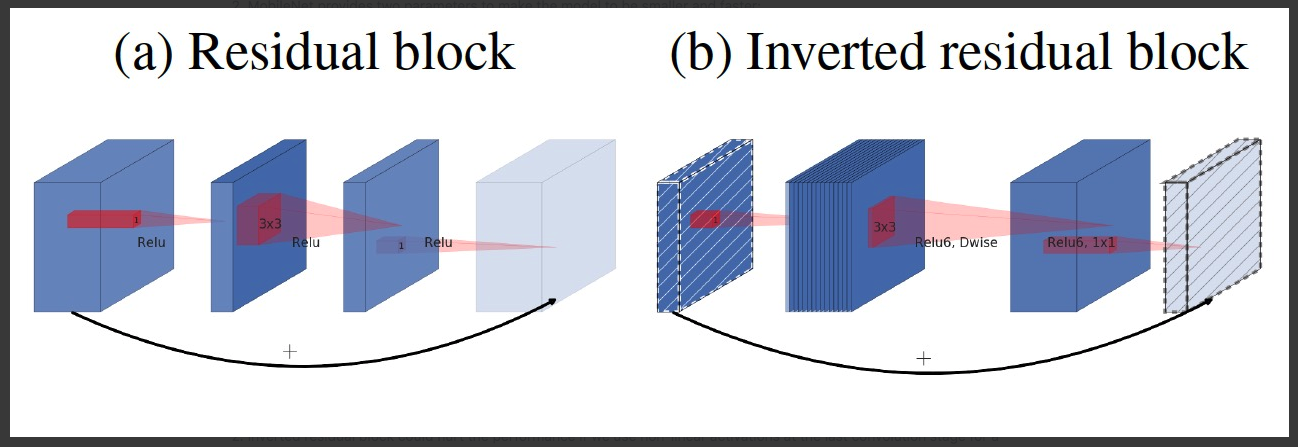
\includegraphics[width=0.6\textwidth]{Images/Modelli/MobileNetV2/Inverted residual block.png}
            \label{MobileNetV2 blocks}
        \end{figure}
        
        \paragraph{Standard residual block}
        Uno\textit{ standard residual block} comprime i canali larghi in canali stretti con convoluzioni $1\times1$ e $3\times3$, e poi li espande di nuovo in canali larghi con convoluzioni $1\times1$.
        
        Si passa da largo - stretto - largo. (Vedere figura \hyperref[MobileNetV2 blocks]{a})
        
        \paragraph{Inverted residual block}
        Un \textit{inverted residual block} utilizza una convoluzione $1\times1$ per espandere i canali e poi aggiungere una depthwise separable convolution per il calcolo successivo. Questo può ridurre significativamente i parametri.
        
        Si passa da stretto - largo - stretto. (Vedere figura \hyperref[MobileNetV2 blocks]{b})
    
        \paragraph{Architettura}
        Di seguito l'architettura del modello MobileNetV2:
            \begin{table}[!h]
                \centering
                \begin{tabular}{|c|c|c|c|c|c|}
                    \hline
                    \textbf{Input} & \textbf{Operator} & \textbf{t} & \textbf{c} & \textbf{n} & \textbf{s}\\
                    \hline \hline
                    \rule[-3mm]{0mm}{8mm}
                    $224^2 \times 3$ & conv2d & - & 32 & 1 & 2\\
                    \hline
                    \rule[-3mm]{0mm}{8mm}
                    $112^2 \times 32 $& bottleneck & 1 & 16 & 1 & 1 \\
                    \hline
                    \rule[-3mm]{0mm}{8mm}
                    $112^2 \times 16$ & bottleneck & 6 & 24 & 2 & 2 \\
                    \hline
                    \rule[-3mm]{0mm}{8mm}
                    $56^2 \times 24$ & bottleneck & 6 & 32 & 3 & 2\\
                    \hline
                    \rule[-3mm]{0mm}{8mm}
                    $28^2 \times 32$ & bottleneck & 6& 64 & 4 & 2\\
                    \hline
                    \rule[-3mm]{0mm}{8mm}
                    $14^2 \times 64 $ & bottleneck & 6 & 96 & 3 & 1\\
                    \hline
                    \rule[-3mm]{0mm}{8mm}
                    $14^2 \times 96$ & bottleneck & 6 & 160 & 3 & 2\\
                    \hline
                    \rule[-3mm]{0mm}{8mm}
                    $7^2 \times 160$ & bottleneck & 6 & 320 & 1 & 1\\
                    \hline
                    \rule[-3mm]{0mm}{8mm}
                    $7^2 \times 320 $ & conv2d $1\times1$ & - & 1280 & 1 & 1\\
                    \hline
                    \rule[-3mm]{0mm}{8mm}
                    $7^2 \times 1280 $ & avgpool $7\times7$ & - & - & 1 & -\\
                    \hline
                    \rule[-3mm]{0mm}{8mm}
                    $1 \times 1 \times 1280$ & conv2d $1\times1$ & - & k & - & \\
                    \hline
                \end{tabular}
                \label{MobileNetV2 Architecture}
            \end{table}
        \newpage
        
        \paragraph{Training and Validation Phase} 
        Di seguito sono riportati i grafici, prodotti durante il lavoro di tesi, raffiguranti le performance del modello, ovvero i valori dell'\textbf{accuracy} e della \textbf{loss} in funzione delle epoche, sia per la fase di \textit{Training} che di \textit{Validation}:
            \begin{figure}[!h]
                \centering
                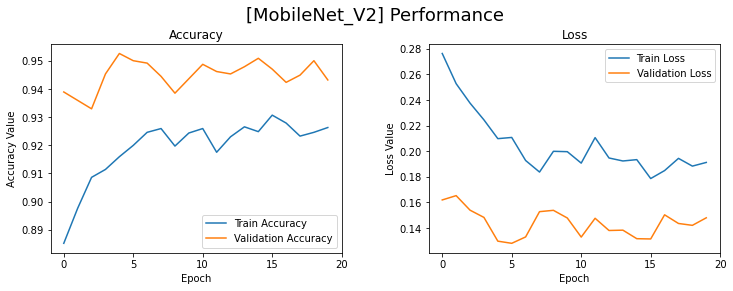
\includegraphics[width=0.7\textwidth]{Images/Modelli/MobileNetV2/MobileNetV2 Pneumonia Performance.png}
                \caption{Performance durante le fasi di \textit{Training} e \textit{Validation} del modello \textit{MobileNetV2} sui Training e Validation datasets di \textit{Chest X-Ray}}
                \label{MobileNetV2 Pneumonia Performance}
            \end{figure}
            
            \begin{figure}[!h]
                \centering
                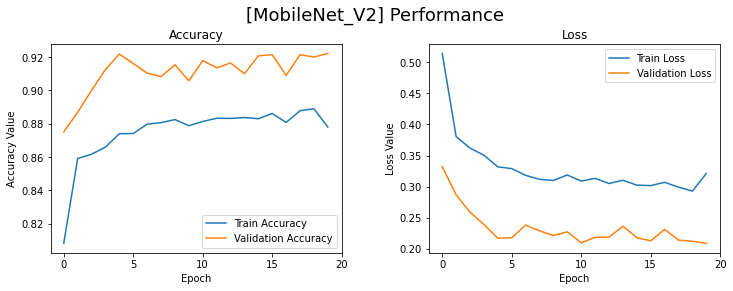
\includegraphics [width=0.7\textwidth]{Images/Modelli/MobileNetV2/MobileNetV2 Brain Performance.png}
                \caption{Performance durante le fasi di \textit{Training} e \textit{Validation} del modello \textit{MobileNetV2} sui Training e Validation datasets di \textit{Brain Tumor MRI}}
                \label{MobileNetV2 Brain Performance}
            \end{figure}
        
        \paragraph{Testing Phase}
        Di seguito si riportano le Confusion Matrices prodotte durante il lavoro di tesi:
            \begin{figure}[!h]
                \centering
                \subfloat[][Confusion Matrix del modello \textit{MobileNetV2} sul Testing dataset di \textit{Chest X-Ray}] {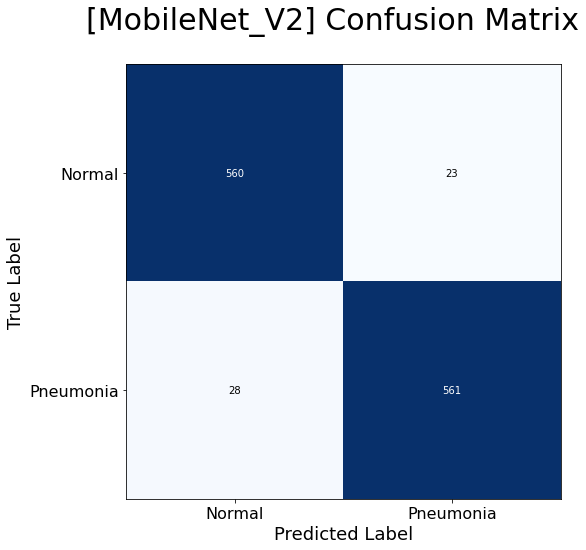
\includegraphics[width=.3\textwidth]{Images/Modelli/MobileNetV2/MobileNetV2 Pneumonia Confusion Matrix.png}} 
                \quad
                \subfloat[][Confusion Matrix del modello \textit{MobileNetV2} sul Testing dataset di \textit{Brain Tumor MRI}] {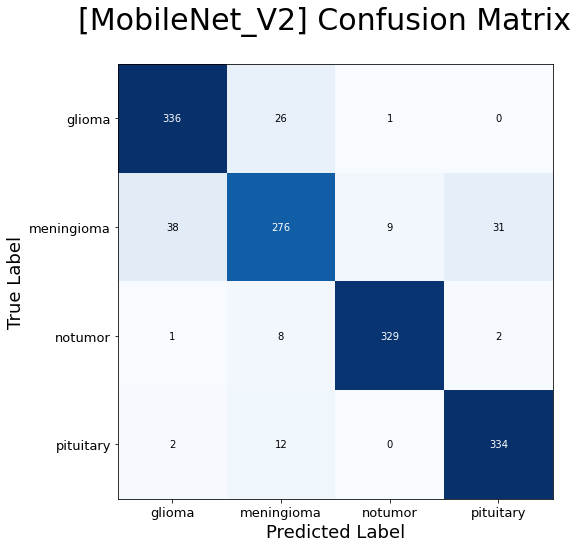
\includegraphics[width=.3\textwidth]{Images/Modelli/MobileNetV2/MobileNetV2 Brain Confusion Matrix.png}}
                \caption{}
                \label{MobileNetV2 Confusion Matrix}
            \end{figure}
        \newpage
        
    \subsection{InceptionV3}
    \label{InceptionV3}
    %[bibl: arXiv:1512.00567]
    Il modello Inception \cite{szegedy2015rethinking}, basandosi sull'uso dei blocchi di costruzione mostrati nella figura \ref{Inception Architecture figures}, mira a cogliere la varietà del dataset evitando un grande consumo di risorse.
    Combinando più filtri di diverse dimensioni allo stesso livello di rete, è possibile catturare informazioni su diverse scale.
        \paragraph{Architettura}
        Di seguito l'architettura del modello InceptionV3:
            \begin{table}[!h]
                \centering
                \begin{tabular}{|c|c|c|}
                    \hline
                    \rule[-3mm]{0mm}{8mm}
                    \textbf{Type} & \textbf{Patch size/stride} & \textbf{Input size}\\
                    & or remarks &\\
                    \hline \hline
                    \rule[-3mm]{0mm}{8mm}
                    conv & 3$\times$3/2 & 299$\times$299$\times$3\\
                    \hline
                    \rule[-3mm]{0mm}{8mm}
                    conv & 3$\times$3/1 & 149$\times$149$\times$32\\
                    \hline
                    \rule[-3mm]{0mm}{8mm}
                    conv padded & 3$\times$3/1 & 147$\times$147$\times$32\\
                    \hline
                    \rule[-3mm]{0mm}{8mm}
                    pool & 3$\times$3/2 & 147$\times$147$\times$64\\
                    \hline
                    \rule[-3mm]{0mm}{8mm}
                    conv & 3$\times$3/1 & 73$\times$73$\times$64\\
                    \hline
                    \rule[-3mm]{0mm}{8mm}
                    conv & 3$\times$3/2 & 71$\times$71$\times$80\\
                    \hline
                    \rule[-3mm]{0mm}{8mm}
                    conv & 3$\times$3/1 & 35$\times$35$\times$192\\
                    \hline
                    \rule[-3mm]{0mm}{8mm}
                    3 $\times$ Inception & As in figure \hyperref[InceptionV3_5]{a} & 35$\times$35$\times$288\\
                    \hline
                    \rule[-3mm]{0mm}{8mm}
                    5 $\times$ Inception & As in figure \hyperref[InceptionV3_6]{b} & 17$\times$17$\times$768\\
                    \hline
                    \rule[-3mm]{0mm}{8mm}
                    2 $\times$ Inception & As in figure \hyperref[InceptionV3_7]{c} & 8$\times$8$\times$1280\\
                    \hline
                    \rule[-3mm]{0mm}{8mm}
                    pool & 8$\times$8 & 8$\times$8$\times$2048\\
                    \hline
                    \rule[-3mm]{0mm}{8mm}
                    linear & logits & 1$\times$1$\times$2048\\
                    \hline
                    \rule[-3mm]{0mm}{8mm}
                    softmax & classifier & 1$\times$1$\times$1000\\
                    \hline
                \end{tabular}
                \label{InceptionV3 Architecture}
            \end{table}
        
            \begin{figure}[!h]
                \centering
                \subfloat[][] {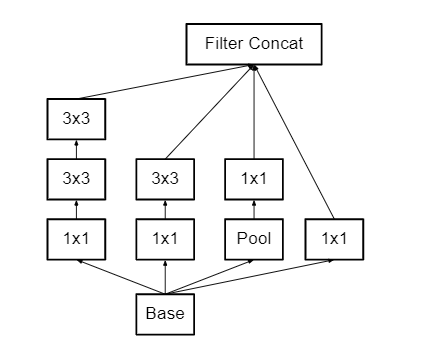
\includegraphics[width=.3\textwidth]{Images/Modelli/InceptionV3/InceptionV3_5.png}} 
                \label{InceptionV3_5}
                \quad
                \subfloat[][] {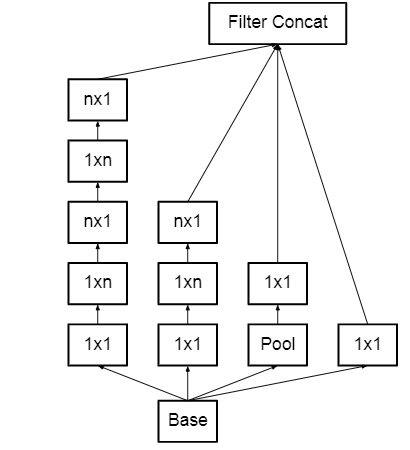
\includegraphics[width=.27\textwidth]{Images/Modelli/InceptionV3/InceptionV3_6.png}} 
                \label{InceptionV3_6}
                \quad
                \subfloat[][] {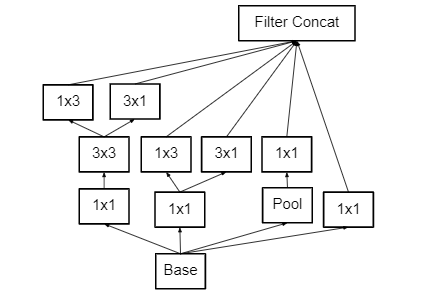
\includegraphics[width=.35\textwidth]{Images/Modelli/InceptionV3/InceptionV3_7.png}}
                \label{InceptionV3_7}
                \caption{}
                \label{Inception Architecture figures}
            \end{figure}
        \newpage
        
        \paragraph{Training and Validation Phase} 
        Di seguito sono riportati i grafici, prodotti durante il lavoro di tesi, raffiguranti le performance del modello, ovvero i valori dell'\textbf{accuracy} e della \textbf{loss} in funzione delle epoche, sia per la fase di \textit{Training} che di \textit{Validation}:
            \begin{figure}[!h]
                \centering
                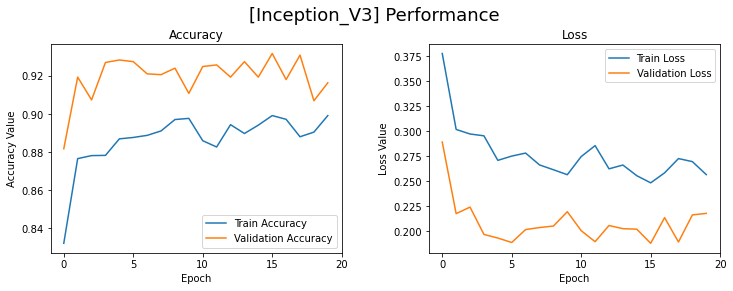
\includegraphics[width=0.7\textwidth]{Images/Modelli/InceptionV3/InceptionV3 Pneumonia Performance.png}
                \caption{Performance durante le fasi di \textit{Training} e \textit{Validation} del modello \textit{InceptionV3} sui Training e Validation datasets di \textit{Chest X-Ray}}
                \label{InceptionV3 Pneumonia Performance}
            \end{figure}
            
            \begin{figure}[!h]
                \centering
                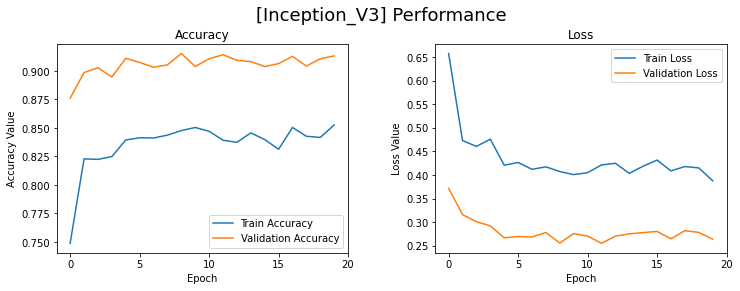
\includegraphics [width=0.7\textwidth]{Images/Modelli/InceptionV3/InceptionV3 Brain Performance.png}
                \caption{Performance durante le fasi di \textit{Training} e \textit{Validation} del modello \textit{InceptionV3} sui Training e Validation datasets di \textit{Brain Tumor MRI}}
                \label{InceptionV3 Brain Performance}
            \end{figure}
        
        \paragraph{Testing Phase}
        Di seguito si riportano le Confusion Matrices prodotte durante il lavoro di tesi:
            \begin{figure}[!h]
                \centering
                \subfloat[][Confusion Matrix del modello \textit{InceptionV3} sul Testing dataset di \textit{Chest X-Ray}] {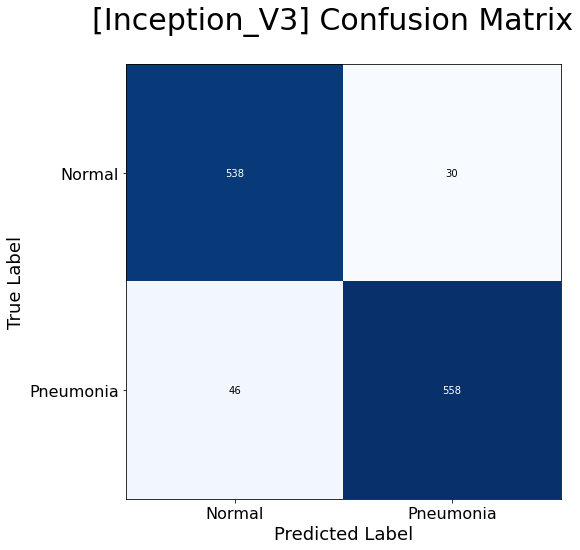
\includegraphics[width=.3\textwidth]{Images/Modelli/InceptionV3/InceptionV3 Pneumonia Confusion Matrix.png}} 
                \quad
                \subfloat[][Confusion Matrix del modello \textit{InceptionV3} sul Testing dataset di \textit{Brain Tumor MRI}] {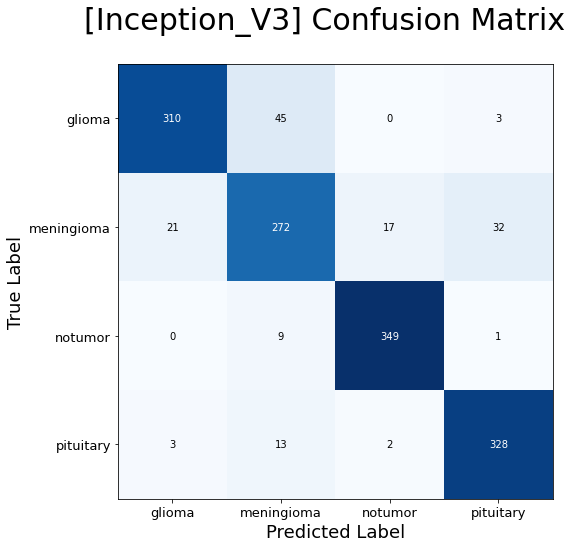
\includegraphics[width=.3\textwidth]{Images/Modelli/InceptionV3/InceptionV3 Brain Confusion Matrix.png}}
                \caption{}
                \label{InceptionV3 Confusion Matrix}
            \end{figure}
    \newpage 
    
\section{Attacchi}
Per eseguire gli attacchi è stata utilizzata la seguente libreria open-source: \\TorchAttacks %[bibl: https://github.com/Harry24k/adversarial-attacks-pytorch]
\cite{kim2020torchattacks}.\\

Si riportano i parametri scelti per i diversi tipi di attacco precedentemente descritti nella sezione \ref{Tecniche di Adversarial Attacks}:
    \begin{table}[!h]
        \centering
        \begin{tabular}{|c|c|}
            \hline
            \rule[-3mm]{0mm}{8mm}
            \textbf{Attack} &\textbf{Parameters used in code} \\ \hline \hline
            \rule[-3mm]{0mm}{8mm}
            FGSM     & $\epsilon=4/255$ \\
            \hline
            \rule[-3mm]{0mm}{8mm}
            BIM      & $\epsilon=4/255,\, \alpha=2/255,\, \text{steps}=100$\\
            \hline
            \rule[-3mm]{0mm}{8mm}
            PGD      & $\epsilon=4/255,\, \alpha=2/255,\, \text{steps}=100$\\
            \hline
            \rule[-3mm]{0mm}{8mm}
            DeepFool & $\text{steps}=50,\, \text{overshoot}=0.02$\\
            \hline
        \end{tabular}
        \caption{}
        \label{Attacks with Parameters}
    \end{table}
    
    La scelta dei parametri è dovuta al grado di percezione del rumore da parte dell'occhio umano. 
    Sono stati scelti i parametri massimi che avrebbero reso la perturbazione impercettibile all'occhio umano.
    Aumentare, anche di poco, i valori dei parametri renderebbe la perturbazione visibile e l'attacco totalmente inefficace perché facilmente rilevabile. 
    
    \newpage
    \subsection{Risultati}
    Di seguito si risportano i risultati degli esperimenti effettuati sugli attacchi durante il lavoro di tesi.
    Si mostra la variazione dell'accuracy dei modelli sulle immagini pulite (No Attacco) e perturbate di entrambi i datasets:
        \begin{table}[!h]
            \centering
            \begin{tabular}{|c||c||c|c|c|c|}
                \hline
                \multicolumn{6}{|c|}{\textbf{Chest X-Ray Dataset}} \rule[-3mm]{0mm}{8mm}\\
                \hline \hline
                \rule[-3mm]{0mm}{8mm}
                \textbf{Modello} & \textbf{No Attacco} & \textbf{FGSM} & \textbf{BIM} & \textbf{PGD} & \textbf{DeepFool} \\
                \hline \hline
                \rule[-3mm]{0mm}{8mm}
                DenseNet121 & 0.9845 & 0.5076  & 0.0000  & 0.0000 & 0.4502\\
                    &  & (-48.44\%) & (-100.0\%) & (-100.0\%) & (-54.27\%)\\
                \hline
                \rule[-3mm]{0mm}{8mm}
                ResNet152   & 0.9811 & 0.4899 & 0.0008 & 0.0017  & 0.4247\\
                    &  & (-50.07\%) & (-99.92\%) & (-99.83\%) & (-56.71\%)\\
                \hline
                \rule[-3mm]{0mm}{8mm}
                VGG19       & 0.9482 & 0.3792  & 0.0000 & 0.0017 & 0.2458\\
                    &  & (-60.01\%) & (-100.0\%) & (-99.82\%) & (-74.08\%)\\
                \hline
                \rule[-3mm]{0mm}{8mm}
                MobileNetV2 & 0.9744 & 0.4780 & 0.0000 & 0.0000 & 0.2534\\
                    &  & (-50.94\%) & (-100.0\%) & (-100.0\%) & (-73.99\%)\\
                \hline
                \rule[-3mm]{0mm}{8mm}
                InceptionV3 & 0.9668 & 0.4899 & 0.0059 & 0.0000 & 0.3446\\
                    &  & (-49.33\%) & (-99.39\%) & (-100.0\%) & (-64.36\%)\\
                \hline
            \end{tabular}
            \caption{Risultati degli attacchi applicati al Testing dataset di \textit{Chest X-Ray}. Ogni cella riporta l'accuracy del modello (riga) sulle immagini perturbate dall'attacco (colonna) e il relativo drop in percentuale rispetto all'accuracy originale.}
            \label{Attacks Results Chest X-Ray}
        \end{table}
        
        \begin{table}[!h]
            \centering
            \begin{tabular}{|c||c||c|c|c|c|}
                \hline
                \multicolumn{6}{|c|}{\textbf{Brain Tumor MRI Dataset}} \rule[-3mm]{0mm}{8mm}\\
                \hline \hline
                \rule[-3mm]{0mm}{8mm}
                \textbf{Modello} & \textbf{No Attacco} & \textbf{FGSM} & \textbf{BIM} & \textbf{PGD} & \textbf{DeepFool} \\
                \hline \hline
                \rule[-3mm]{0mm}{8mm}
                DenseNet121 & 0.9554 & 0.3137 & 0.0007 & 0.0000 & 0.3334 \\
                 & & (-67.17\%) & (-99.93\%) & (-100.0\%) & (-65.10\%)\\
                \hline
                \rule[-3mm]{0mm}{8mm}
                ResNet152   & 0.9332 & 0.4273 & 0.0014 & 0.0000 & 0.4374 \\
                 & & (-54.21\%) & (-99.85\%) & (-100.0\%) & (-53.13\%)\\
                \hline
                \rule[-3mm]{0mm}{8mm}
                VGG19       & 0.9197 & 0.3650 & 0.0156 & 0.0044 & 0.3593 \\
                 & & (-60.31\%) & (-98.30\%) & (-99.52\%) & (-60.93\%)\\
                \hline
                \rule[-3mm]{0mm}{8mm}
                MobileNetV2 & 0.9277 & 0.2789 & 0.0007 & 0.0000 & 0.1564 \\
                 & & (-69.94\%) & (-99.92\%) & (-100.0\%) & (-83.14\%)\\
                \hline
                \rule[-3mm]{0mm}{8mm}
                InceptionV3 & 0.9160 & 0.4598 & 0.0000 & 0.0000 & 0.3659 \\
                 & & (-49.80\%) & (-100.0\%) & (-100.0\%) & (-60.05\%)\\
                \hline
            \end{tabular}
            \caption{Risultati degli attacchi applicati al Testing dataset di \textit{Brain Tumor MRI}. Ogni cella riporta l'accuracy del modello (riga) sulle immagini perturbate dall'attacco (colonna) e il relativo drop in percentuale rispetto all'accuracy originale.}
            \label{Attacks Results Brain Tumor MRI}
        \end{table}
    
    \newpage
    Tutti i 5 modelli considerati sono risultati altamente vulnerabili agli adversarial attacks scelti, con conseguenti diminuzioni significative nell'accuracy dei modelli per entrambi i datasets. 
    
    Gli attacchi più efficaci sono stati BIM e PGD, i quali hanno comportato un calo dell'accuracy, per tutti i modelli e i datasets, superiore al $98\%$.
    Da notare che, a parità di valori assegnati ai parametri ($\epsilon=4/255,\, \alpha=2/255,\, \text{steps}=100$), l'attacco PGD risulta, anche se di poco, più forte di BIM.
    
    Il modello più debole per la classificazione binaria (due sole classi) è VGG19, mentre per la classificazione multiclass (con 3 o più classi) è MobileNetV2. I due modelli, se attaccati, non riescono a raggiungere rispettivamente il 40\% e il 30\% di accuracy. 
    Inoltre, gli attacchi hanno un tasso di successo maggiore sul testing dataset di \textit{Brain Tumor MRI}. Si osserva che, a parità di perturbazioni, l'accuratezza dei vari modelli sugli adversarial examples diminuisce all'aumentare del numero di classi. Ciò significa che i datasets multiclass sono più vulnerabili rispetto a quelli binari.
    
    \newpage
    Si riportano di seguito alcuni esempi di classificazione errata:
        \begin{figure}[!h]
            \centering
            \subfloat[][8 esempi con rispettive classi reali e predizioni del modello \textit{DenseNet121} su immagini perturbate con l'attacco PGD del Testing dataset di \textit{Brain Tumor MRI}] {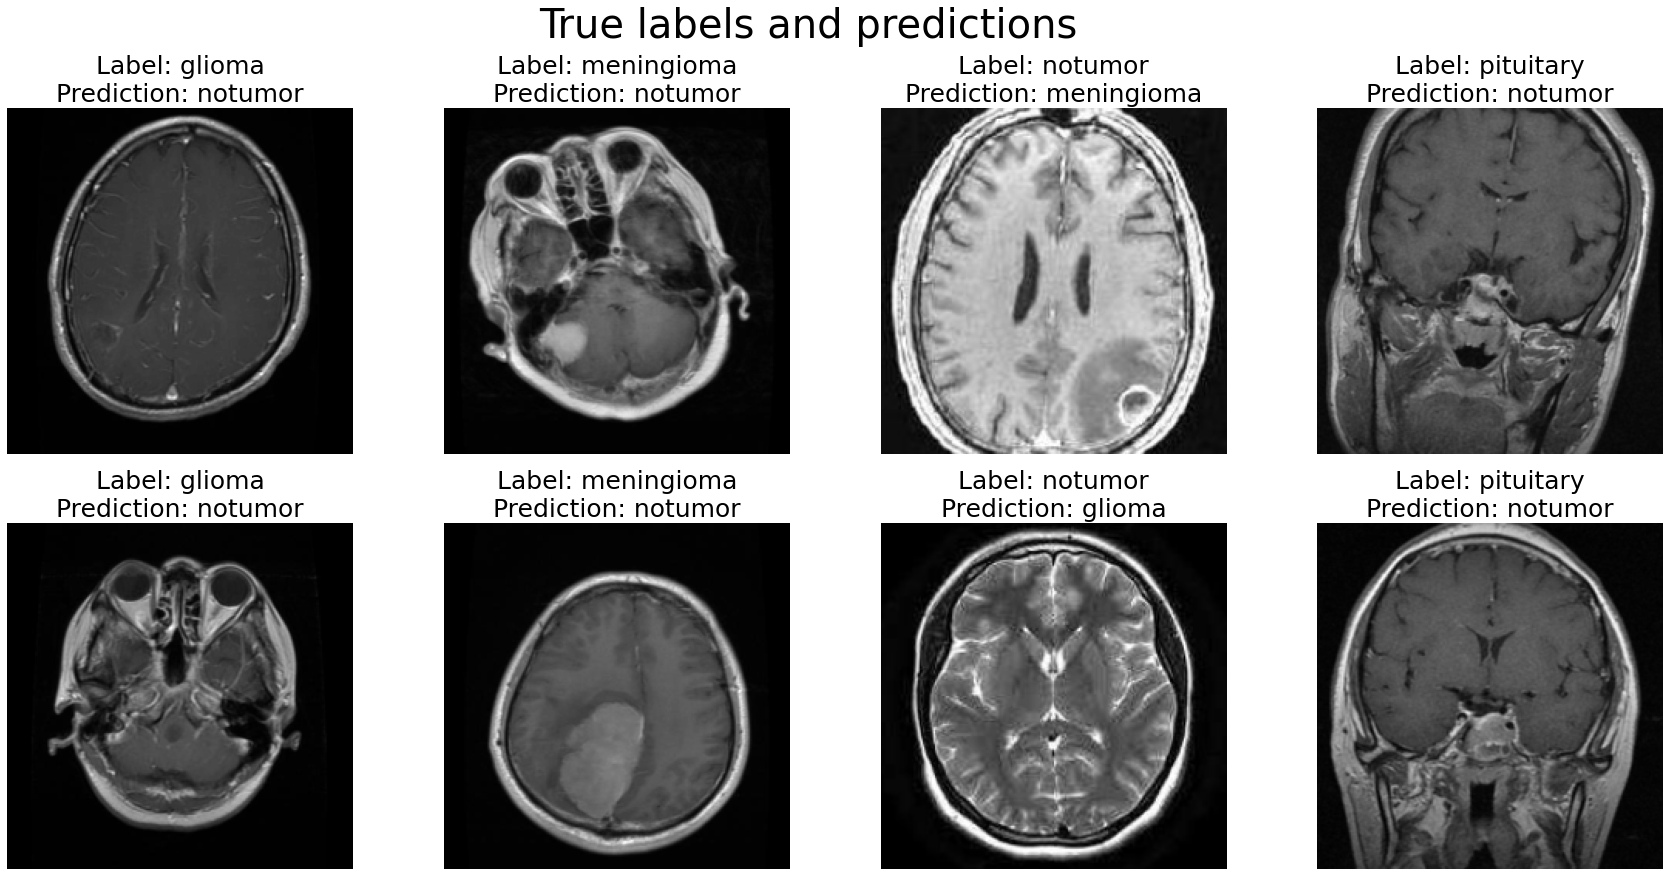
\includegraphics[width=\textwidth]{Images/Esempi attacchi/Brain MRI/Densenet121 Brain PGD 8 True&Predictions.png}}
            \quad
            \subfloat[][10 esempi con rispettive classi reali e predizioni del modello \textit{DenseNet121} su immagini perturbate con l'attacco PGD del Testing dataset di \textit{Chest X-Ray}] {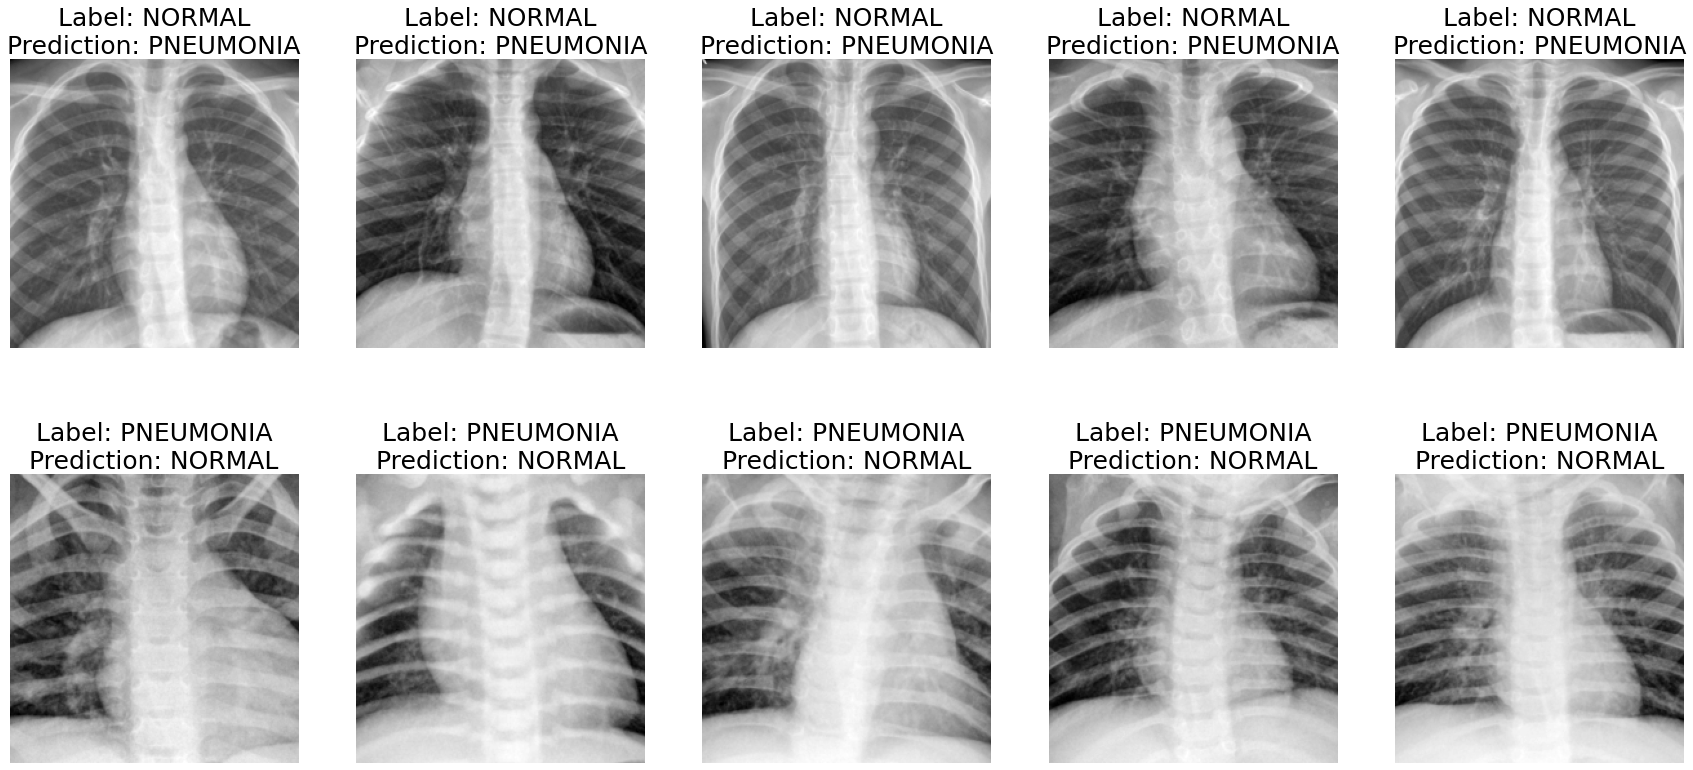
\includegraphics[width=\textwidth]{Images/Esempi attacchi/Pneumonia/DenseNet121 Pneumonia PGD 10 True&Predictions.png}} 
            \caption{}
            \label{DenseNet121 wrong predictions}
        \end{figure}
    
    \newpage
    Di seguito alcune immagini che raffigurano le perturbazioni e gli adversarial examples prodotti dagli attacchi sul Testing dataset di \textit{Chest X-Ray}:
        
        \begin{figure}[!h]
            \centering
            
            \quad
            \subfloat[][Originale] {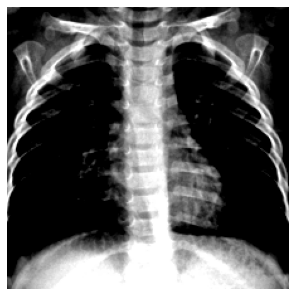
\includegraphics[width=.25\textwidth]{Images/Esempi attacchi/Pneumonia/FGSM_Clean.png}} 
            \quad
            \subfloat[][Perturbata\\ (FGSM)] {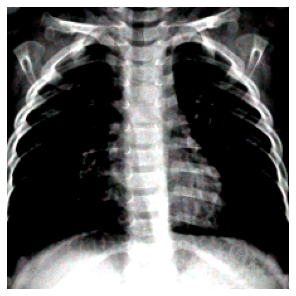
\includegraphics[width=.25\textwidth]{Images/Esempi attacchi/Pneumonia/FGSM_Perturbated.png}}
            \quad
            \subfloat[][Perturbazione\\ (FGSM)] {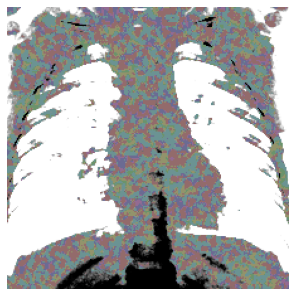
\includegraphics[width=.25\textwidth]{Images/Esempi attacchi/Pneumonia/FGSM_Noise.png}}
            
            \quad
            \subfloat[][Originale] {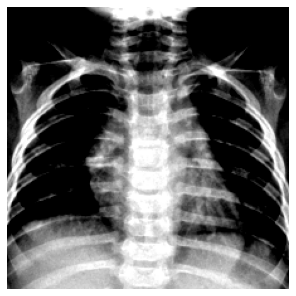
\includegraphics[width=.25\textwidth]{Images/Esempi attacchi/Pneumonia/BIM_Clean.png}} 
            \quad
            \subfloat[][Perturbata\\ (BIM)] {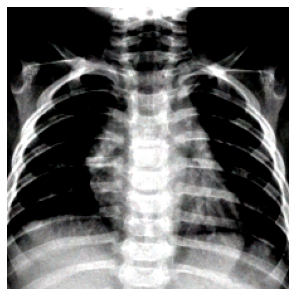
\includegraphics[width=.25\textwidth]{Images/Esempi attacchi/Pneumonia/BIM_Perturbated.png}}
            \quad
            \subfloat[][Perturbazione\\ (BIM)] {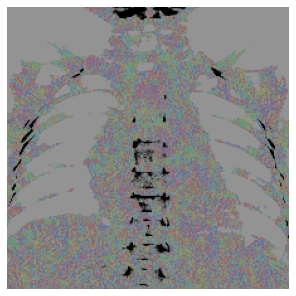
\includegraphics[width=.25\textwidth]{Images/Esempi attacchi/Pneumonia/BIM_Noise.png}}
            
            \quad
            \subfloat[][Originala] {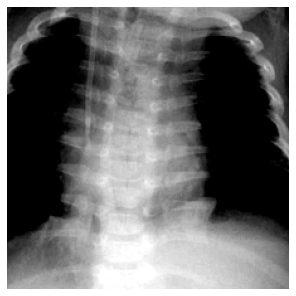
\includegraphics[width=.25\textwidth]{Images/Esempi attacchi/Pneumonia/PGD_Clean.png}} 
            \quad
            \subfloat[][Perturbata\\ (PGD)] {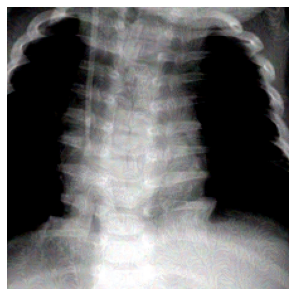
\includegraphics[width=.25\textwidth]{Images/Esempi attacchi/Pneumonia/PGD_Perturbated.png}}
            \quad
            \subfloat[][Perturbazione\\ (PGD)] {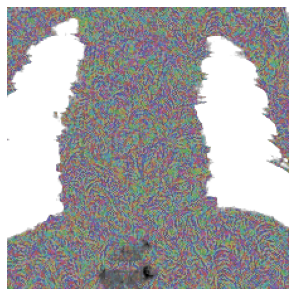
\includegraphics[width=.25\textwidth]{Images/Esempi attacchi/Pneumonia/PGD_Noise.png}}
            
            \quad
            \subfloat[][Originale] {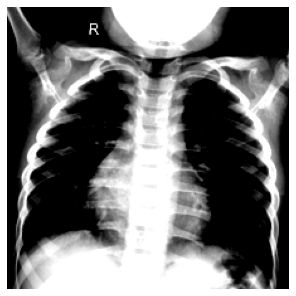
\includegraphics[width=.25\textwidth]{Images/Esempi attacchi/Pneumonia/DeepFool_Clean.png}} 
            \quad
            \subfloat[][Perturbata\\ (DeepFool)] {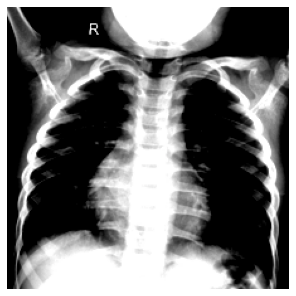
\includegraphics[width=.25\textwidth]{Images/Esempi attacchi/Pneumonia/DeepFool_Perturbated.png}}
            \quad
            \subfloat[][Perturbazione\\ (DeepFool)] {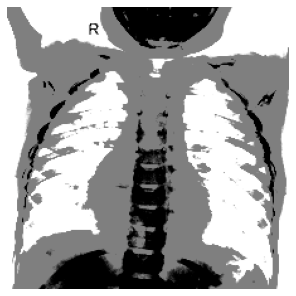
\includegraphics[width=.25\textwidth]{Images/Esempi attacchi/Pneumonia/DeepFool_Noise.png}}
            
            \caption{Esempi di perturbazioni create per ingannare il modello \textit{DenseNet121} su immagini del Testing dataset di \textit{Chest X-Ray}. Ogni riga rappresenta un attacco diverso e si compone di 3 immagini: l'immagine originale e pulita, l'adversarial example corrispondente, la perturbazione aggiunta alla prima immagine per produrre la seconda.}
            \label{Attacks Examples Chest X-Ray}
        \end{figure}
    
    \newpage    
    Di seguito alcune immagini che raffigurano le perturbazioni e gli adversarial examples prodotti dagli attacchi sul Testing dataset di \textit{Brain Tumor MRI}:
        \begin{figure}[!h]
            \centering
            
            \quad
            \subfloat[][Originale] {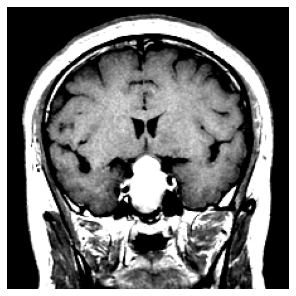
\includegraphics[width=.25\textwidth]{Images/Esempi attacchi/Brain MRI/FGSM_Clean.png}} 
            \quad
            \subfloat[][Perturbata\\ (FGSM)] {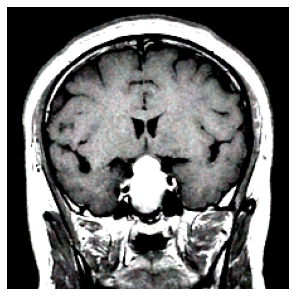
\includegraphics[width=.25\textwidth]{Images/Esempi attacchi/Brain MRI/FGSM_Perturbated.png}}
            \quad
            \subfloat[][Perturbazione\\ (FGSM)] {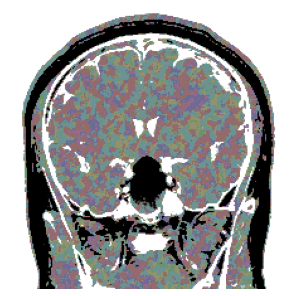
\includegraphics[width=.25\textwidth]{Images/Esempi attacchi/Brain MRI/FGSM_Noise.png}}
            
            \quad
            \subfloat[][Originale] {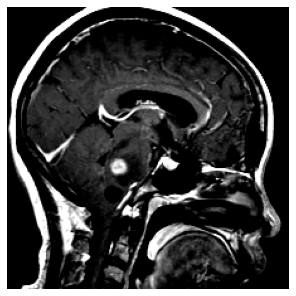
\includegraphics[width=.25\textwidth]{Images/Esempi attacchi/Brain MRI/BIM_Clean.png}} 
            \quad
            \subfloat[][Perturbata\\ (BIM)] {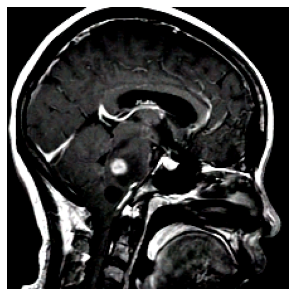
\includegraphics[width=.25\textwidth]{Images/Esempi attacchi/Brain MRI/BIM_Perturbated.png}}
            \quad
            \subfloat[][Perturbazione\\ (BIM)] {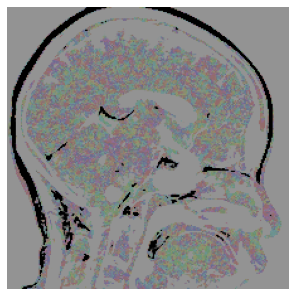
\includegraphics[width=.25\textwidth]{Images/Esempi attacchi/Brain MRI/BIM_Noise.png}}
            
            \quad
            \subfloat[][Originale] {\includegraphics[width=.25\textwidth]{Images/Esempi attacchi/Brain MRI/PGD_Clean.png}} 
            \quad
            \subfloat[][Perturbata\\ (PGD)] {\includegraphics[width=.25\textwidth]{Images/Esempi attacchi/Brain MRI/PGD_Perturbated.png}}
            \quad
            \subfloat[][Perturbazione\\ (PGD)] {\includegraphics[width=.25\textwidth]{Images/Esempi attacchi/Brain MRI/PGD_Noise.png}}
            
            \quad
            \subfloat[][Originale] {\includegraphics[width=.25\textwidth]{Images/Esempi attacchi/Brain MRI/DeepFool_Clean.png}} 
            \quad
            \subfloat[][Perturbata\\ (DeepFool)] {\includegraphics[width=.25\textwidth]{Images/Esempi attacchi/Brain MRI/DeepFool_Perturbated.png}}
            \quad
            \subfloat[][Perturbazione\\ (DeepFool)] {\includegraphics[width=.25\textwidth]{Images/Esempi attacchi/Brain MRI/DeepFool_Noise.png}}
            
            \caption{Esempi di perturbazioni create per ingannare il modello \textit{DenseNet121} su immagini del Testing dataset di \textit{Brain Tumor MRI}. Ogni riga rappresenta un attacco diverso e si compone di 3 immagini: l'immagine originale e pulita, l'adversarial example corrispondente, la perturbazione aggiunta alla prima immagine per produrre la seconda.}
            \label{Attacks Examples Brain Tumor MRI}
        \end{figure}